\documentclass[11pt]{article}

%	packages
\usepackage{tikz}
\usepackage{pgfplots}
\usepackage{authblk}
\usepackage{amsmath}
\usepackage{amssymb} 
\usepackage{caption}
\usepackage{graphicx}
\usepackage[hypertexnames=false,colorlinks=true,linkcolor=blue,citecolor=blue]{hyperref}
\usepackage[numbers,comma,square,sort&compress]{natbib}
\usepackage[a4paper,text={6.5in,10in},centering]{geometry}
\usepackage{subcaption}
%	code syntax higlighting
\usepackage{listings}
\usepackage{color}
\usepackage{textcomp}
\definecolor{listinggray}{gray}{0.9}
\definecolor{lbcolor}{rgb}{0.9,0.9,0.9}
% C++ = [Visual]C++ ; matlab = matlab
\lstset{
	backgroundcolor=\color{lbcolor},
	tabsize=4,
	rulecolor=,
	language=java,
	keywordstyle=\bfseries\ttfamily\color[rgb]{0,0,1},
	identifierstyle=\ttfamily,
	commentstyle=\color[rgb]{0.133,0.545,0.133},
	stringstyle=\ttfamily\color[rgb]{0.627,0.126,0.941},
	showstringspaces=false,
	basicstyle=\small,
	%numberstyle=\footnotesize,
	%numbers=left,
	stepnumber=1,
	numbersep=10pt,
	tabsize=2,
	breaklines=true,
	prebreak = \raisebox{0ex}[0ex][0ex]{\ensuremath{\hookleftarrow}},
	breakatwhitespace=false,
	aboveskip={1.5\baselineskip},
  columns=fixed,
  upquote=true,
  extendedchars=true,
 frame=single,
% backgroundcolor=\color{lbcolor},
}


%	figures
\graphicspath{{eps/}{pdf/}{../Figures/}}
%\setcaptionmargin{0.25in}
\def\captionfont{\itshape\small}
\def\captionlabelfont{\upshape\small}

%	counters
\makeatletter\@addtoreset{equation}{section}\makeatother
\renewcommand{\theequation}{\arabic{section}.\arabic{equation}}


%%%%%%%%%%%%%%%%%%%%%%%%%%%%%%%%%%%%%%%%%%%%%%%%%%%%%%%%%%%%%%%%%%%%%%%%%%%%

\begin{document}

\title{Equation-free analysis of agent-based models:\\Fire spreading in a Forest}

%\author[1]{Spencer A. Thomas}
\author{Spencer A. Thomas}
\author{David J.B. Lloyd}
\author{Anne C. Skeldon}
%\affil[1]{\small Department of Mathematics, Evolution and Resilience of Industrial Ecosystems (ERIE), University of Surrey, Guildford, GU2 7XH, UK}
\affil{\small Department of Mathematics, Evolution and Resilience of Industrial Ecosystems (ERIE), University of Surrey, Guildford, GU2 7XH, UK}
\date{\today}
\maketitle


%%%%%%%%%%%%%%%%%%%%%%%%%%%%%%%%%%%%%%%%%%%%%
% stochastic double well
%%%%%%%%%%%%%%%%%%%%%%%%%%%%%%%%%%%%%%%%%%%%%

\section{The Model: An Overview}

This model is available in the NetLogo \cite{Netlogo} model library and simulates the spread of fire through a forest represented by a 2D lattice where the fire is started on one side of the forest \cite{Fire}, see Fig.~\ref{fig:fire}. The model contains only one parameter, the density of trees in the forest. How far the fire spreads depends on the density, but also has a dependence on the (randomly) initialised location of the trees. Here a fire dies out rapidly in sparse forests, or burn the majority of trees in a dense forest. In this model a fire can spread in any direction in the 2D lattice, but assumes there is no wind, so a fire can only spread from one tree to another unburned tree.

\begin{figure}[h!]
        \centering
        		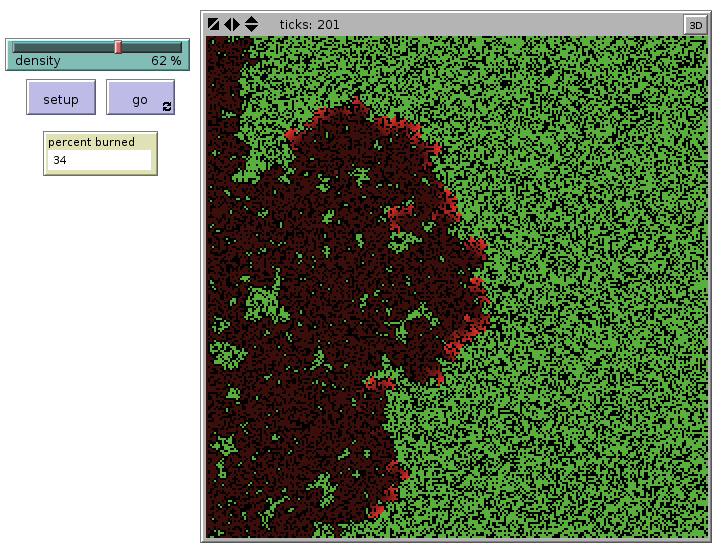
\includegraphics[width=0.8\textwidth]{../Figures/FireInterface}
            \caption{NetLogo Interface for the Fire model. The only tunable parameter is forest density. \label{fig:fire}}
\end{figure}

\section{The Model: Details} 
\label{sec:details}

The density of the forest, $\rho$, is the only controllable parameter in this simple model. The level of noise in this model is low, however the number of trees burnt for a given forest density will vary between runs. We analyse the equilibrium state in this model between initial density $\rho$ in the forest and the percentage of trees burnt,
	\begin{equation}
		F(\rho, \kappa^\ast) = \kappa^\ast~,
	\end{equation}
	where $\kappa$ is the ratio of burned trees after $\tau$ and initial number of trees.


\section{Requirements of the User}
The user defined settings in the input file are given below. 
\begin{lstlisting}
String NetlogoFile = "netlogo/Fire.nlogo"; 
String[] systemParameters = {"set density"};
double[] param = {10.0}; 
String[] Measure	= {"(burned-trees / initial-trees) * 100.0"};
String[] LiftOperator = {"set density"}; 
double[] Initial	= {10.0}; 
boolean isSystemInitialised = false;  
\end{lstlisting}		
Here the continuation parameters is the density of trees in the forest after each ensemble has been simulated the measure of the system us the percentage of tress burned from the initial population.


\section{Outcome of Equation-free Analysis}
The results of the continuation are shown in Fig.~\ref{fig:fireDynamics}. This illustrates the existence of a critical parameter with a non-linear threshold, a common feature in complex systems \cite{Fire}. Moreover this threshold is over a narrow range of forest density, which can be set between 0 and 100. Investigating this model by simply running simulations could easily observe a linear dependence due to a coarse interval in $\rho$ or due to the noise in the system which is largest during the transition, see Fig.~\ref{fig:firefireDynamics The initial forest density is illustrates in the insets of Fig.~\ref{fig:fireDynamics}(a) across the range of $\rho$. Also included are the distributions of simulation results illustrating the relatively low variance at low and high forest densities, where as variance is large when the density is around 60\% and leads to larger standard errors for the fixed points in Fig.~\ref{fireDynamics}(a) at this density.  

 	\begin{figure}[h]
        \centering
        \subfloat[]{
        		\begin{tikzpicture}
        			%\node[] at (0,0) {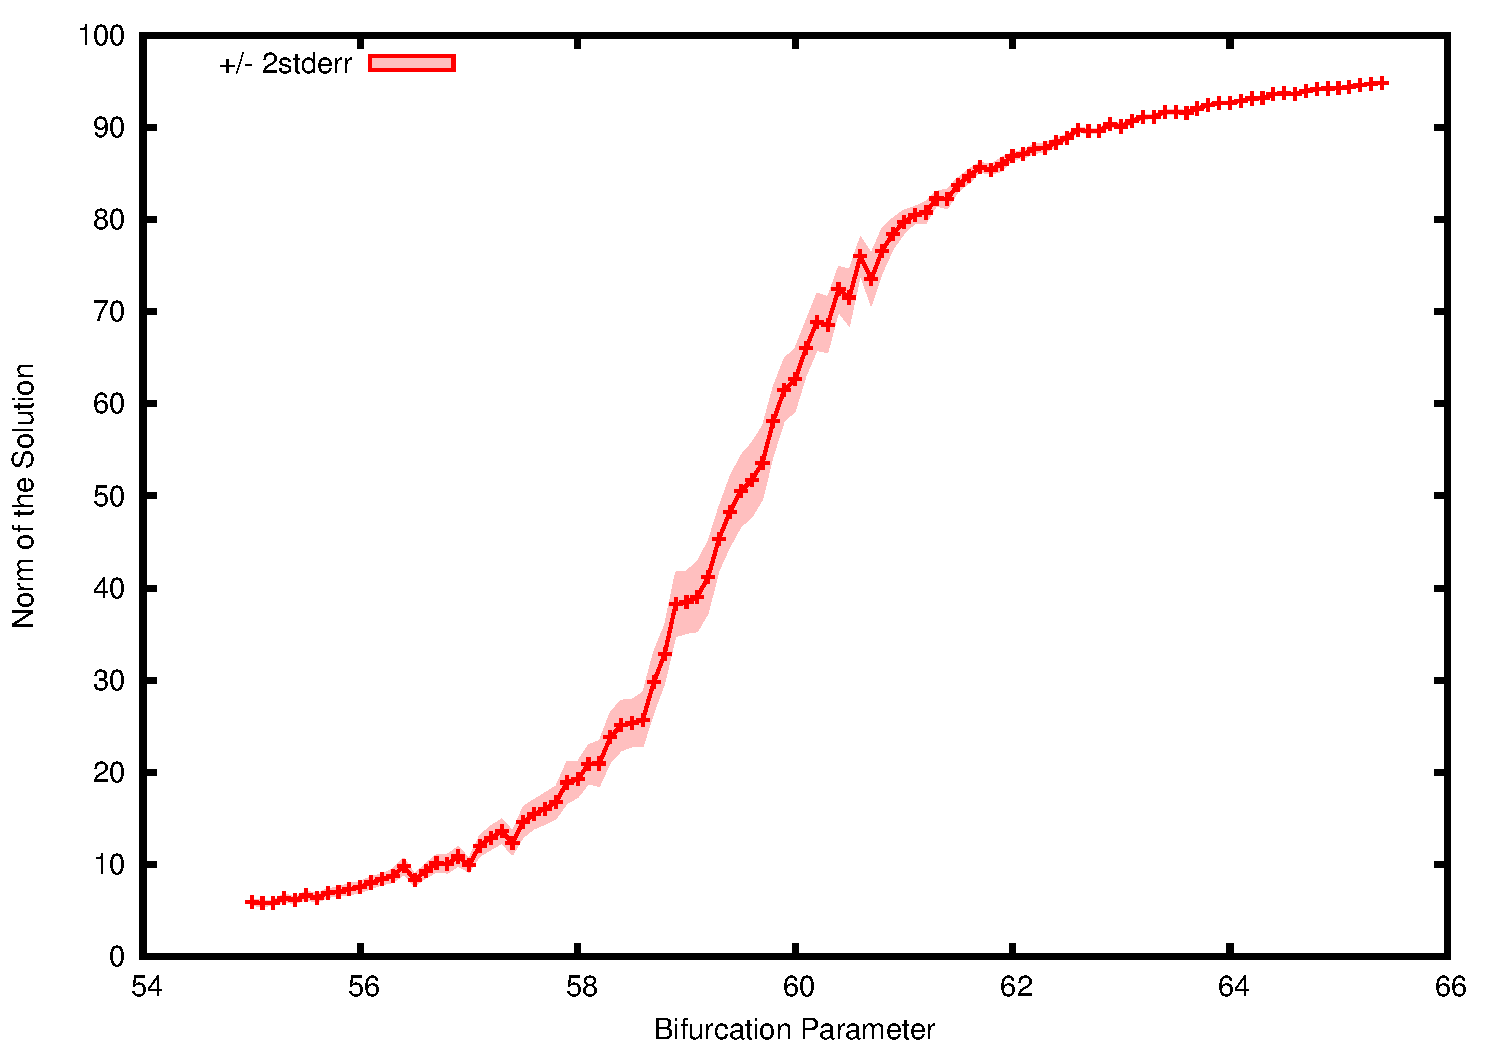
\includegraphics[width=0.41\textwidth, trim=2.1cm 1.5cm 0cm 0cm, clip=true]{FIRE}};
        		\node[] at (0,0.2) {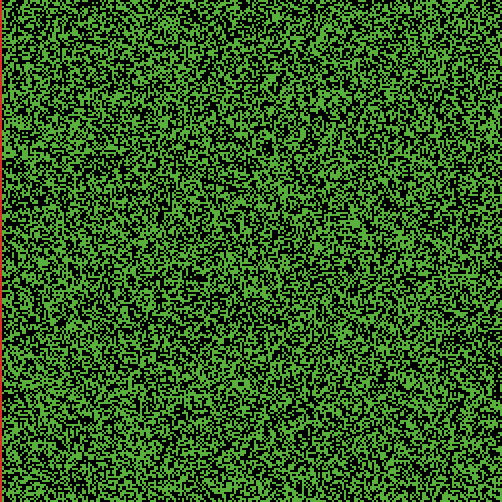
\includegraphics[width=0.075\textwidth]{FireMIDview.png}};
        		\node[] at (2.25,1.55) {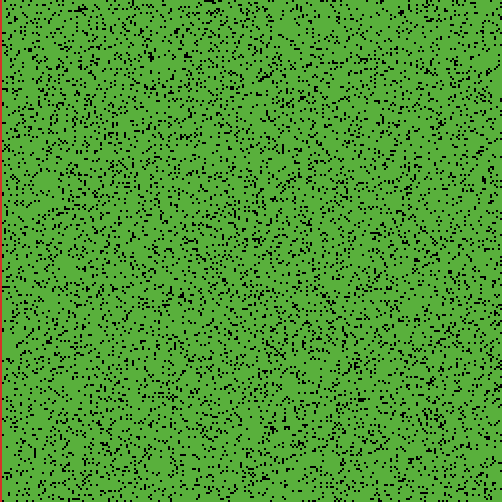
\includegraphics[width=0.075\textwidth]{FireHIGHview.png}};
        		\node[] at (-2,-1.5) {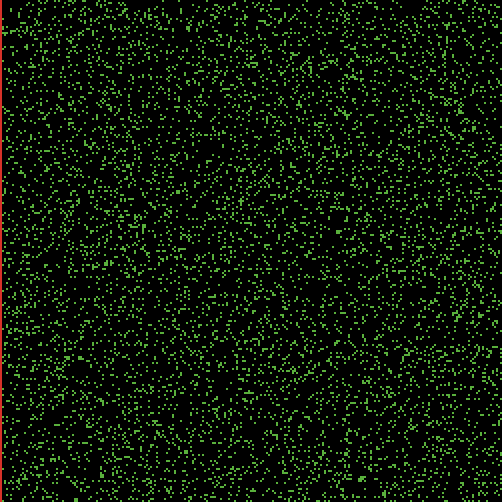
\includegraphics[width=0.075\textwidth]{FireLOWview.png}};
        		\node[] (plot) at (0,0) {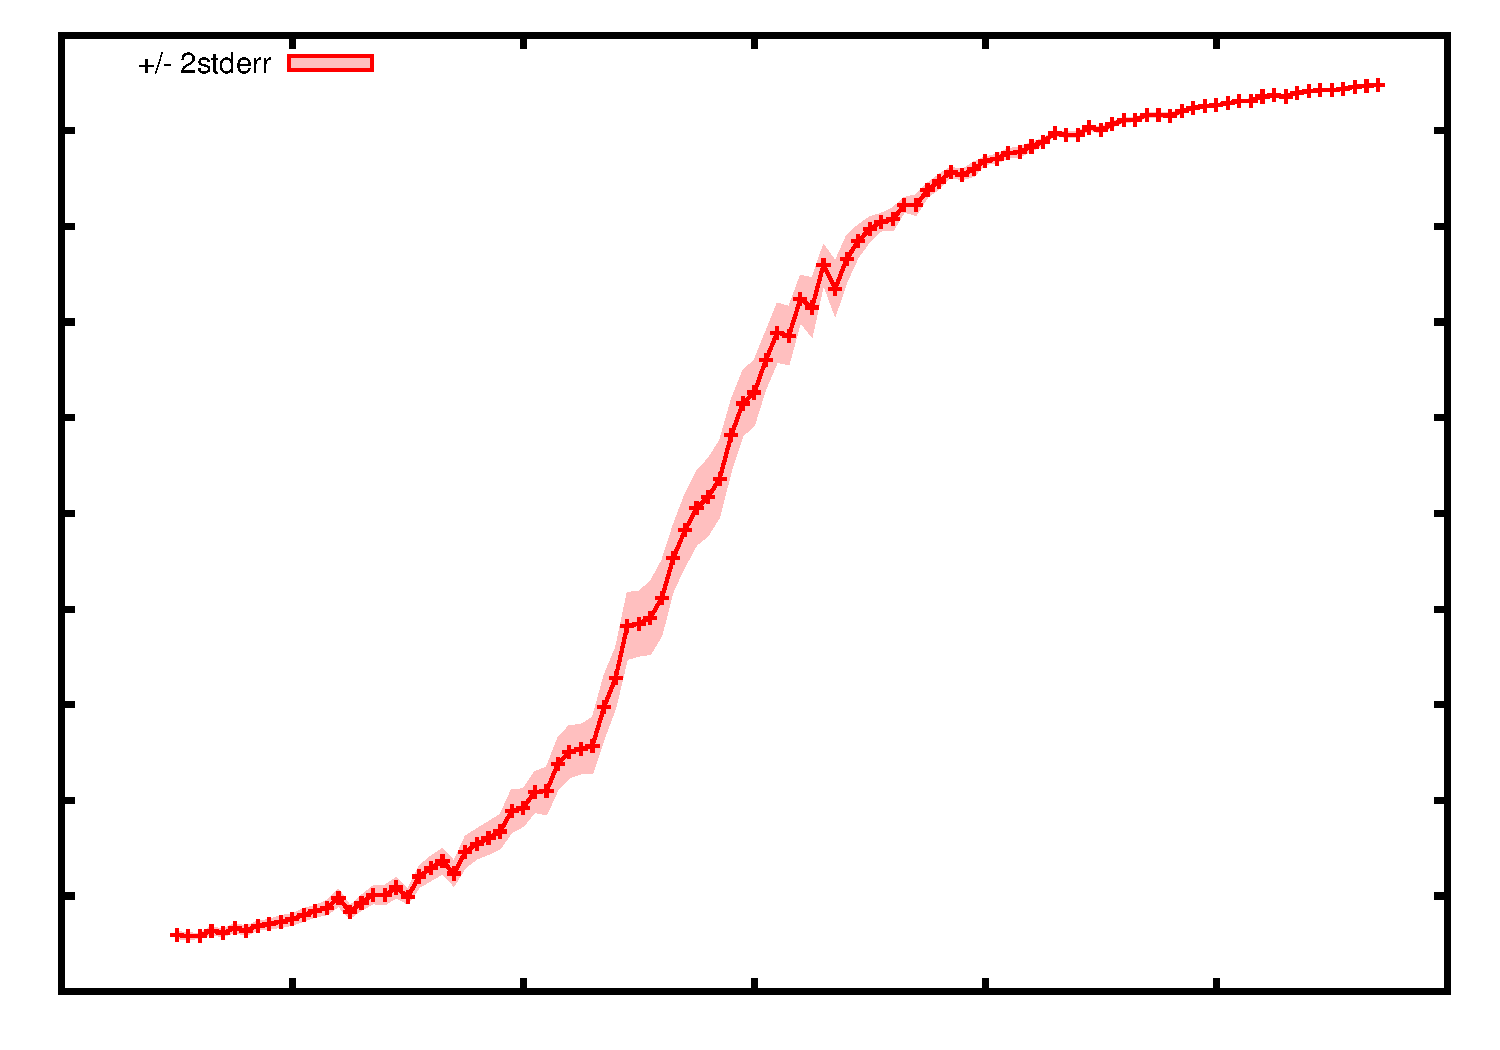
\includegraphics[width=0.41\textwidth]{Fire2}};
			%\begin{axis}[enlargelimits=false, axis on top, axis equal image]        			
       		%	\addplot graphics [xmin=54,xmax=66,ymin=0,ymax=100] {Fire2};
        		%\end{axis}
        		\end{tikzpicture}
        } 
        \subfloat[]{
        		\begin{tikzpicture}
        			\node[] at (0,0) {\includegraphics[width=0.4\textwidth, page=10, trim=1cm 0.75cm 0cm 0cm, clip=true]{FireDistribution}};
        			\node[] at (0,0) {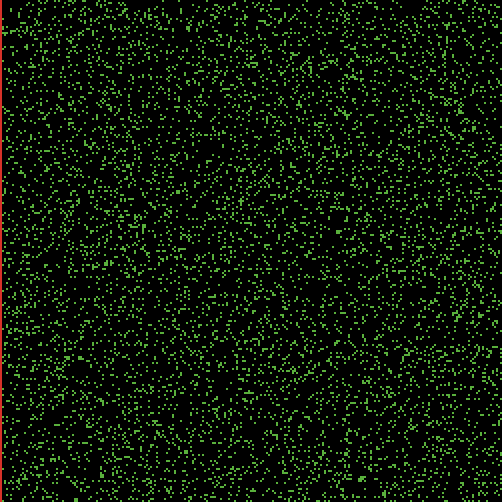
\includegraphics[width=0.15\textwidth]{FireLOWview.png}};
        		\end{tikzpicture}
        } \\
        \subfloat[]{
        		\begin{tikzpicture}
        			\node[] at (0,0) {\includegraphics[width=0.4\textwidth, page=50, trim=1cm 0.75cm 0cm 0cm, clip=true]{FireDistribution}};
        			\node[] at (0,0) {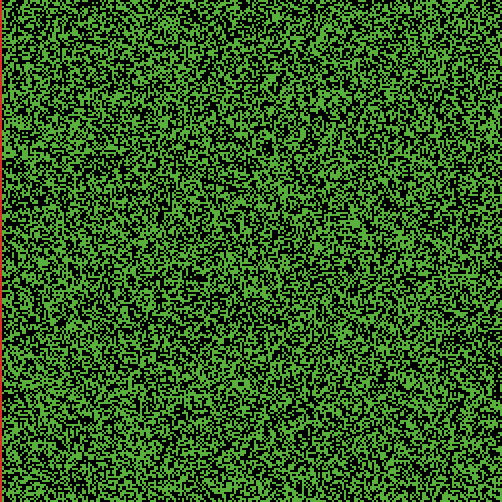
\includegraphics[width=0.15\textwidth]{FireMIDview.png}};
        		\end{tikzpicture}
        } 
        \subfloat[]{
        		\begin{tikzpicture}
        			\node[] at (0,0) {\includegraphics[width=0.4\textwidth, page=62, trim=1cm 0.75cm 0cm 0cm, clip=true]{FireDistribution}};
        			\node[] at (0,0) {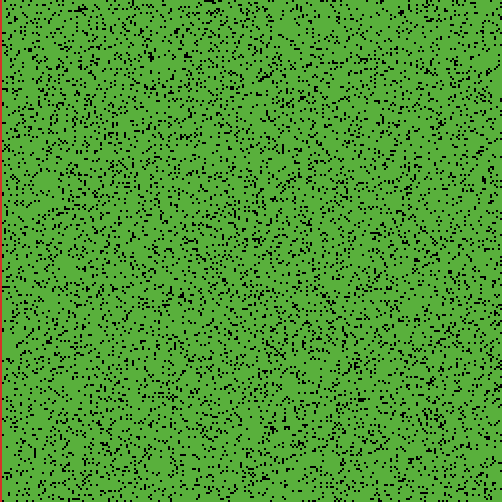
\includegraphics[width=0.15\textwidth]{FireHIGHview.png}};
        		\end{tikzpicture}
        } 
        \caption{Continuation of the NetLogo Fire model \cite{Fire} with (a) parameter dependence curve and (b)-(d) distribution of realisations after simulation. \label{fig:fireDynamics}}
	\end{figure} 
 
\section{Further Reading}

The following table contains a reference list for further reading on the topic contained in this method and example. 
\begin{center}
\begin{tabular}{|l|c|}
\hline
Topic									&	Reference \\ \hline
Introduction to bifurcation analysis		&	\cite{Meunier1988}	\\
Introduction to continuation 			&	\cite{Doedel1991,Allgower1990,Rheinboldt2000,Krauskopf2007} \\ 
Introduction to equation-free methods	&	\cite{Theodoropoulos2000,Kevrekidis2003,Kevrekidis2009} \\
\hline
\end{tabular}
\end{center}



\section*{Acknowledgments}
{The support of the UK Engineering and Physical Sciences Research Council for programme grant EP/H021779/1 (Evolution and Resilience of Industrial Ecosystems (ERIE)) is gratefully acknowledged.}
 
 
\begin{thebibliography}{10}  
\bibitem{Netlogo}
{\sc U. Wilensky}, 
{\it NetLogo},
Center for Connected Learning and Computer-Based Modeling, Northwestern University, Evanston, IL,
http://ccl.northwestern.edu/netlogo/,
1999

\bibitem{Fire}
{\sc U. Wilensky}, 
{\it NetLogo Fire model},
Center for Connected Learning and Computer-Based Modeling, Northwestern University, Evanston, IL,
http://ccl.northwestern.edu/netlogo/models/Fire,
1997

\bibitem{Meunier1988}
{\sc C. Meunier and A. D. Verga},
{\it Noise and Bifurcations}
J. Stat. Phys., 1988, 50(1-2), pp 345-375

\bibitem{Doedel1991}
{\sc E. Doedel, H. B. Keller and J. P. Kernevez},
{\it Numerical Analysis And Control of Bifurcation Problems (I) Bifurcation in Finite Dimensions}
Int. J. Bifurcation Chaos, 1991, 493(3), pp 493-520

\bibitem{Allgower1990}
{\sc E. L. Allgower and K. Georg},
{\it Numerical Continuation Methods, An Introduction}
Springer-Verlag Berlin Heidelberg 1990

\bibitem{Rheinboldt2000}
{\sc W. C. Rheinboldt},
{\it Numerical continuation methods: a perspective}
Journal of Computational and Applied Mathematics, 200, 124, pp 229-244

\bibitem{Krauskopf2007}
{\sc B. Krauskopf, H. M. Osinga and J. Gal\`{a}n-Vioque (Eds.)},
{\it Numerical Continuation Methods for Dynamical Systems}
Springer 2007

\bibitem{Theodoropoulos2000}
{\sc C. Theodoropoulos, Y. H. Qian and I. G. Kevrekidis IG}
{\it Coarse stability and bifurcation analysis using time-steppers: a reaction-diffusion example}
Proc. Natl. Acad. Sci. 2000, 97, pp 9840-9845

\bibitem{Kevrekidis2003}
{\sc I. G. Kevrekidis et al.} 
{\it Equation-free, coarse-grained multiscale computation: enabling microscopic simulators to perform system-level tasks}
Comm. Math. Sci. 2003, 1, pp 715-762 

\bibitem{Kevrekidis2009}
{\sc I. G. Kevrekidis and G. Samaey},
{\it Equation-Free Multiscale Computation: Algorithms and Applications},
Annual Review of Physical Chemistry, 2009, 60(1), pp 321-344


\end{thebibliography} 

\end{document} 

